\documentclass[brazil, 10pt]{beamer}
\usepackage[T1]{fontenc}
\usepackage[utf8]{inputenc}
\usepackage{lmodern}
\usepackage[brazilian]{babel}
\usepackage{hyperref}
\usepackage{listings}
\usetheme{JuanLesPins}

\makeatletter
\setbeamertemplate{footline}
{
  \leavevmode%
  \hbox{%
  \begin{beamercolorbox}[wd=\paperwidth,ht=2.25ex,dp=1ex,right]{date in head/foot}%
    \insertframenumber\hspace*{2ex} 
  \end{beamercolorbox}}%
  \vskip0pt%
}
\makeatother

\title{Implementação do Método de Integração Numérica Runge-Kutta em GPGPU para Aplicações Científicas}
\author{Giancarlo Rigo\\
        Rafael Reggiani Manzo}

\begin{document}
\maketitle

\section{Introdução}
\begin{frame}
  \frametitle{}
  \framesubtitle{}
  \begin{Large}
  \begin{center}
  \textbf{Introdução}
  \end{center}
  \end{Large}
\end{frame}

\begin{frame}
  \frametitle{Na prática}
  
  \begin{itemize}
    \item Aplicações para visualização de imagens por difusão de tensores (\textit{DTI - Diffusion Tensors Images}) costumam oferecer uma funcionalidade chamada de tractografia (\textit{fiber tracking});
    \item Por trás desta funcionalidade estão diversas instâncias independentes de problemas de valor inicial (ou integração numérica de uma equação diferencial ordinária);
    \item A solução destes problemas pode ser aproximada pelo algoritmo de Runge-Kutta;
    \item Porém, quando temos centenas de instâncias do problema, os cálculos podem levar também centenas de segundos. O que torna impossível sua implementação em tempo real;
    \item Para tonar possível os cálculos em tempo real implementações em GPU são uma solução já utilizada. 
  \end{itemize}
  
\end{frame}

\subsection{Base matemática}
\begin{frame}
  \frametitle{Problemas de Valor Inicial\footnote{PRESS, William H. et al. \textit{Numerical Recipes in C}}}
  \framesubtitle{ou \textit{IVP (Initial Value Problem)}}

  Dados:
  \begin{itemize}
    \item Equação Diferencial Ordinária (EDO): $f(x, y(x)) = \frac{dy}{dx} $
    \item Lista de pontos iniciais: $ (x_{0}, y_{0}),...,(x_{n},y_{n}) $
    \item Tamanho de passo $ h $
  \end{itemize}
   
  Para cada ponto inicial $ (x_{i}, y_{i}) $ queremos calcular o valor de $ y $ em $ x_{i} + h $ 
\end{frame}

\begin{frame}
  \frametitle{Método de Integração Numérica Runge-Kutta\footnote{PRESS, William H. et al. \textit{Numerical Recipes in C}}}
  \framesubtitle{Ordem 2}
  \begin{itemize}
    \item O algoritmo é uma generalização do método de Euler para aproximação de solução de EDOs usando séries de Taylor
    \item Para ordem 2 temos a seguinte expressão, onde $ k_{1} $ e $ k_{2} $ são variáveis auxiliares:
  \end{itemize}
 
  $ k_{1} = h\ldotp f(x_{n},y_{n}) $\\
  $ k_{2} = h\ldotp f(x_{n} + \frac{h}{2},y_{n} + \frac{k_{1}}{2}) $\\
  $ y_{n+1} = y_{n} + k_{2} + O(h^{3}) $ 
  
\end{frame}

\begin{frame}
  \frametitle{Método de Integração Numérica Runge-Kutta\footnote{PRESS, William H. et al. \textit{Numerical Recipes in C}}}
  \framesubtitle{Ordem 4}
  \begin{itemize}
    \item Para ordem 4 temos a seguinte expressão, onde $ k_{1} $, $ k_{2} $, $ k_{3} $ e $ k_{4} $ são variáveis auxiliares:
  \end{itemize}
 
  $ k_{1} = h\ldotp f(x_{n},y_{n}) $\\
  $ k_{2} = h\ldotp f(x_{n} + \frac{h}{2},y_{n} + \frac{k_{1}}{2}) $\\
  $ k_{3} = h\ldotp f(x_{n} + \frac{h}{2},y_{n} + \frac{k_{2}}{2}) $\\
  $ k_{4} = h\ldotp f(x_{n} + h,y_{n} + k_{3}) $\\
  $ y_{n+1} = y_{n} + \frac{k_{1}}{6} + \frac{k_{2}}{3} + \frac{k_{3}}{3} + \frac{k_{4}}{6} + O(h^{5}) $ 
  
\end{frame}

\begin{frame}
  \frametitle{Campos Vetoriais}

  \begin{itemize}
    \item Representam a discretização de uma ou mais EDOs
    \item $ x_{i} + h $ pode não estar definido no campo
    \item Podem ser muito complexos (várias EDOs misturadas no mesmo campo)
  \end{itemize}
\end{frame}

\subsection{GPGPU}

\begin{frame}
  \frametitle{GPGPU}
  \framesubtitle{General Purpose Computing on Graphics Processing Units}
  
  Computação de propósito geral na unidade de processamento gráfico.
  
  \begin{itemize}
    \item As GPUs são utilizadas principalmente para processamento gráfico, mas descobriu-se seu poder de processamento é muito interessante também para outros tipos de processamento que envolvam cálculos e sejam altamente paralelizáveis.
    \item Uma NVIDIA GeForce GTX 690 possui mais de 3000 núcleos de processamento (\textit{CUDA Cores}) a aproximadamente 900MHz cada e 4GB de memória dedicada\footnote{\href{http://www.nvidia.com.br/object/geforce-gtx-690-br.html}{Catálogo NVIDIA}}.
  \end{itemize}
  
  Então este é um ambiente bastante propenso para implementarmos nosso algoritmo e obtermos uma implementação do método de Runge-Kutta em tempo real.
\end{frame}

\begin{frame}
  \frametitle{Paralelismo}
  \framesubtitle{Conceito}
  
  \begin{itemize}
    \item Em computação, paralelismo consiste em executar trechos diferentes de um algoritmo ao mesmo tempo ao invés de fazê-lo sequencialmente;
    \item Por exemplo, podemos pensar na soma de oito números;
    \item Sequencialmente, se cada soma consome uma unidade de tempo, esta soma tomaria 6 unidades;
    \item Porém, realizando as somas duas a duas em paralelo reduzimos este tempo pela metade;
  \end{itemize}
\end{frame}

\begin{frame}
  \frametitle{Paralelismo}
  \framesubtitle{Exemplo ilustrado}

  2 + 2 + 2 + 2 + 2 + 2 + 2 + 2

  \begin{columns}
    \begin{column}{.3\textwidth}
      \textbf{Soma sequencial}
    
      \begin{enumerate}
        \item 2 + 2 = 4;
        \item 4 + 2 = 6;
        \item 6 + 2 = 8;
        \item 8 + 2 = 10;
        \item 10 + 2 = 12;
        \item 12 + 2 = 14;
        \item 14 + 2 = 16.
      \end{enumerate}
    \end{column}
    \begin{column}{.7\textwidth}
      \textbf{Soma em paralelo}
    
      \begin{enumerate}
        \item (2+2) + (2+2) + (2+2) + (2+2) = 4 + 4 + 4 + 4;
        \item (4+4) + (4+4) = 8 + 8;
        \item (8+8) = 16.
      \end{enumerate}
    \end{column}
  \end{columns}
\end{frame}
\begin{frame}
  \frametitle{Implementação de algoritmos gerais em GPU}
  \begin{itemize}
    \item No inicío era feito em termos de operações gráficas (produto de matrizes de textura por exemplo)
    \item Com o surgimento da linguagem Cg isso se tornou mais plausível, mas ela ainda é uma linguagem baseada no C que é convertida em termos de DirectX ou shaders do OpenGL.
    \item Percebendo a necessidade de algo mais próximo às linguagens de propósito geral, surgiram outras duas linguagens CUDA e OpenCL que podem ser utilizadas como extensões das linguagens C, C++ e Fortran.
  \end{itemize}
\end{frame}

\begin{frame}
  \frametitle{Comparação teórica}

\begin{columns}
  \begin{column}{.5\textwidth}
    CUDA
    
    \begin{itemize}
      \item Propriedade da NVIDIA.
      \item Apenas para GPUs NVIDIA (apesar de seguir o padrão LLVM, só existe compilador para GPUs NVIDIA).
      \item Alto acoplamento ao código (é possível mesclar CUDA com outras linguagens no mesmo arquivo fonte).
      \item Tem maior conhecimento do hardware permitindo otimizações específicas para este.
    \end{itemize}
  \end{column}
  \begin{column}{.5\textwidth}
    OpenCL    
    
    \begin{itemize}
      \item A marca é propriedade da Apple (desenvolveu a primeira versão), mas é desenvolvido pelo Khronos Group, um consórcio de empresas que atualmente inclui AMD, ARM, Intel e NVIDIA e outras empresas.
      \item Executado em GPUs e CPUs de qualquer fabricante desde que com os drivers apropriados.
    \end{itemize}
  \end{column}
\end{columns}
\end{frame}

\section{Motivação}
\begin{frame}
  \begin{Large}
  \begin{center}
  \textbf{Motivação}
  \end{center}
  \end{Large}
\end{frame}

\begin{frame}
  \frametitle{Objetivos}

  \begin{itemize}
    \item Protótipos em C++, CUDA e OpenCL;
    \item Realizar testes para comprovar se os desempenhos são os esperados;
    \item Protótipo utilizando a biblioteca VTK.
  \end{itemize}
\end{frame}

\section{Metodologia}
\begin{frame}
  \frametitle{}
  \framesubtitle{}
  \begin{Large}
  \begin{center}
  \textbf{Metodologia}
  \end{center}
  \end{Large}
\end{frame}

\begin{frame}
  \frametitle{Adapatação a campos vetoriais}
  \framesubtitle{Quanto as EDOs}
  
  \begin{itemize}
    \item Temos vetores que podemos interpretar como a direção da reta tangente na direção da função que desejamos aproximar.
    \item O que nos leva a seguinte expressão para o RK4, por exemplo:

    $k_{1} = h\ldotp (\alpha ,\beta ,\gamma)$\\
    $k_{2} = \frac{k_{1}}{2} + h\ldotp (\alpha ,\beta ,\gamma)$\\
    $k_{3} = \frac{k_{2}}{2} + h\ldotp (\alpha ,\beta ,\gamma)$\\
    $k_{4} = k_{3} + h\ldotp (\alpha ,\beta ,\gamma )$\\
    $(x_{n+1}, y_{n+1}, z_{n+1}) = (x_{n}, y_{n}, z_{n}) + \frac{k_{1}}{6} + \frac{k_{2}}{3} + \frac{k_{3}}{3} + \frac{k_{4}}{6}$
    
    \item Onde $ (x_{n}, y_{n}, z_{n}) $ é um ponto inicial, $(\alpha ,\beta ,\gamma)$ é o vetor associado a este ponto e $ (x_{n+1}, y_{n+1}, z_{n+1}) $ é o ponto resultante do método
  \end{itemize}


\end{frame}

\begin{frame}
  \frametitle{Adapatação a campos vetoriais}
  \framesubtitle{Quanto a natureza dos campos vetoriais}

  \begin{itemize}
    \item Em pontos nos quais não há um vetor associado, fazemos a interpolação (\textit{Trilinear interpolation}).
    \item No limite do campo não teremos todos os pontos necessários para a interpolação. Então usamos o mais simples possível que é buscar o vizinho mais próximo (\textit{Nearest Neighbour}).
  \end{itemize}
\end{frame}

\section{Aplicações}
\begin{frame}
  \frametitle{}
  \framesubtitle{}
  \begin{Large}
  \begin{center}
  \textbf{Aplicações}
  \end{center}
  \end{Large}
\end{frame}

\subsection{Trajetórias de fibras de substância branca cerebral utilizando ressonância magnética}
\begin{frame}
  \frametitle{Tractografia}
  \framesubtitle{Imagens Por Difusão de Tensores}
  
  \begin{itemize}
    \item São obtidas através do resultado da análise de como prótons interagem com as moléculas, geralmente água;
    \item Permitindo a análise do processo de difusão destas;
    \item Estas imagens podem ter diferentes dimensões em quantidade de pontos e espaçamentos entre estes pontos, dependendo de como foi calibrado o equipamento de ressonância magnética;
    \item Uma resolução usual para imagens de um coração é a de 256 pontos no eixo x, outros 256 no eixo y e mais 128 pontos no eixo z, com espeçamento por volta de 5mm entre cada ponto.
  \end{itemize}

  
\end{frame}

\begin{frame}
  \frametitle{Tractografia}
  \framesubtitle{Fibra}
  \textbf{Definição de fibra}
  \begin{itemize}
    \item Existem imagens de ressonância magnética por difusão de tensores que resultam em campos vetoriais que representam caminhos nervosos ou musculares;
    \item Reconstrução tridimensional de trajetórias do trato como extensão natural do campo vetorial obtido através de uma ressonância magnética\footnote{Mori, S. and van Zijl, P. C. M. (2002), Fiber tracking: principles and strategies – a technical review. NMR Biomed., 15: 468–480. doi: 10.1002/nbm.781}.
  \end{itemize}
  
\end{frame}

\begin{frame}
  \frametitle{Tractografia}
  \framesubtitle{Quais fibras calcular}
  \begin{itemize}
    \item Geralmente são calculadas a partir de um ou mais pontos iniciais em ambos os sentidos (o mesmo processo é feito para o campo vetorial oposto).
    \item Este conjunto de um ou mais pontos é chamado de região de interesse\footnote{Mori, S. and van Zijl, P. C. M. (2002), Fiber tracking: principles and strategies – a technical review. NMR Biomed., 15: 468–480. doi: 10.1002/nbm.781}.
  \end{itemize}
\end{frame}

\begin{frame}
  \frametitle{Paralelizável}
  
  \begin{itemize}
    \item Cada ponto inicial e cada direção são instâncias independentes (o ponto de uma fibra, idealmente, não é influenciado por outra fibra) do problema que podem ser resolvidas concorrentemente.
    \item Então temos um problema altamente paralelizável que envolve múltiplas operações de ponto flutuante ideal para ser tratado na GPU.
  \end{itemize}
\end{frame}

\subsection{Implementação}
\begin{frame}
  \frametitle{O que foi feito}

  \begin{itemize}
    \item Implementações do RK2 e RK4 em C++, CUDA e OpenCL;
    \item Testes comparativos do método em GPU e CPU;
    \item Visualização do resultado do método em OpenGL;
    \item Visualização do resultado do método através da VTK;
    \item Resultado do método pode ser exportado para o GNUPlot.
  \end{itemize}
\end{frame}

\begin{frame}
  \frametitle{Kernel RK4}
  \framesubtitle{CUDA}
  
  \lstinputlisting[language=C++, basicstyle=\tiny]{code/rk4_kernel.cu}
\end{frame}

\begin{frame}
  \frametitle{Kernel RK4}
  \framesubtitle{OpenCL}
  
  \lstinputlisting[language=C++, basicstyle=\tiny]{code/rk4_kernel.cl}
\end{frame}

\begin{frame}
  \frametitle{Testes de performance}
  \framesubtitle{Processamento}
  
  \begin{columns}
    \begin{column}{.5\textwidth}
      \begin{figure}[!h]
        \begin{center}
          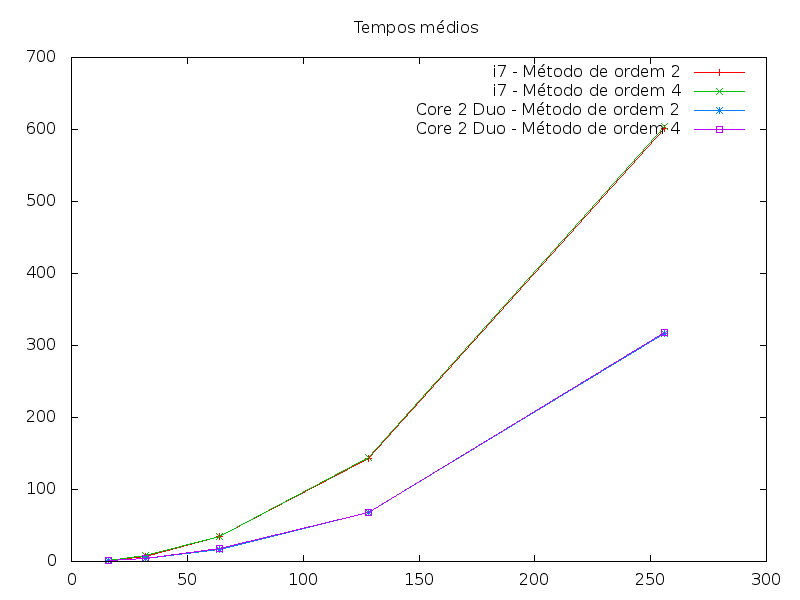
\includegraphics[width=1.1\textwidth, height=.7\textwidth]{img/cpu-means.png}
          \label{fig:cpu-means}
          \caption{Média dos tempos de processamento em CPU pela quantidade de pontos iniciais}
        \end{center}
      \end{figure}
    \end{column}
    \begin{column}{.5\textwidth}
      \begin{figure}[!h]
        \begin{center}
          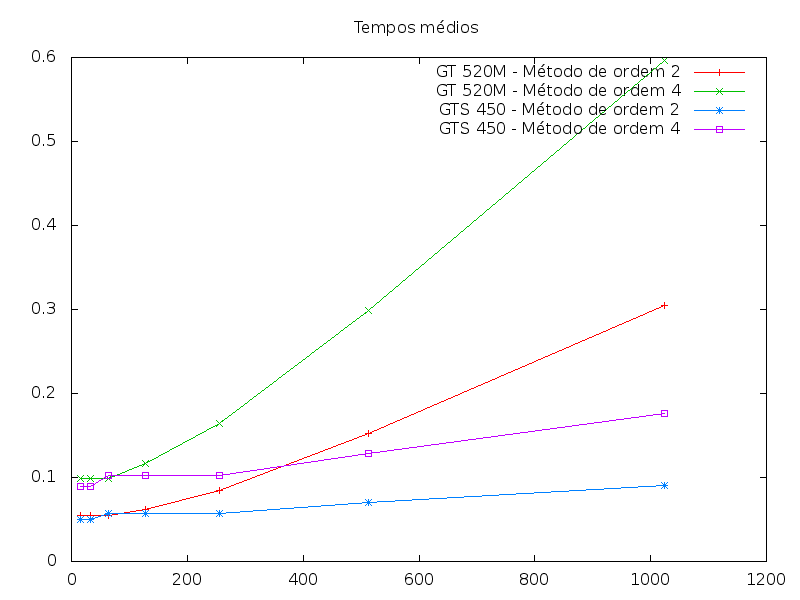
\includegraphics[width=1.1\textwidth, height=.7\textwidth]{img/gpu-means-double.png}
          \label{fig:cpu-means}
          \caption{Média dos tempos de processamento em GPU pela quantidade de pontos iniciais}
        \end{center}
      \end{figure}
    \end{column}
  \end{columns}
\end{frame}

\begin{frame}
  \frametitle{Testes de performance}
  \framesubtitle{Memória}
  
  \begin{columns}
    \begin{column}{.5\textwidth}
      \begin{itemize}
        \item Em CPU, apesar de o problema crescer exponencialmente o tempo gasto em operações em memória é constante, devido ao se barramento dedicado;
        \item Por outro lado, na GPU este é o maior consumo de tempo, com crescimento linear (gráfico ao lado);
        \item Porém a soma dos tempos de processamento com o de operações em memória ainda é muito mais vantajoso para a GPU.
      \end{itemize}
    \end{column}
    \begin{column}{.5\textwidth}
      \begin{figure}[!h]
        \begin{center}
          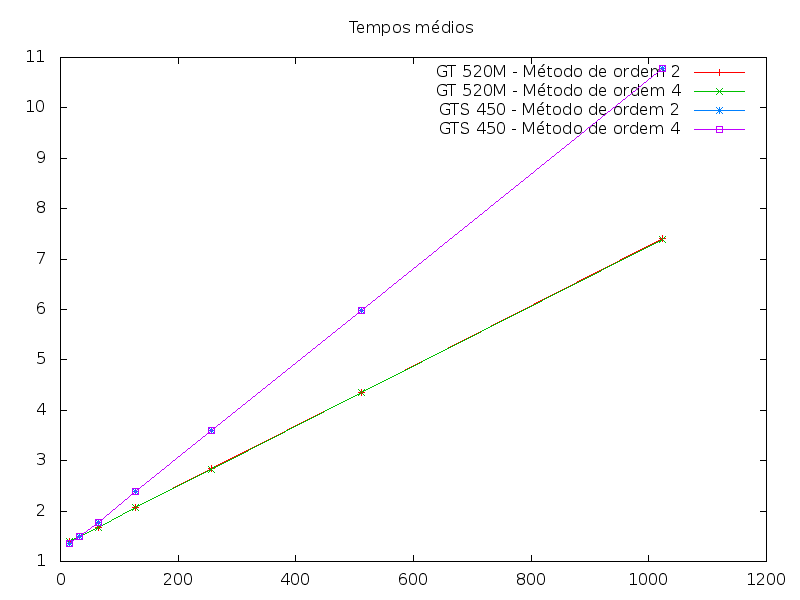
\includegraphics[width=1.1\textwidth, height=.7\textwidth]{img/gpu-memo-means-double.png}
          \label{fig:cpu-means}
          \caption{Média dos tempos de operações memória para GPU pela quantidade de pontos iniciais}
        \end{center}
      \end{figure}
    \end{column}
  \end{columns}

\end{frame}

\begin{frame}
  \frametitle{Visualização}
  \framesubtitle{GNUPlot}
  
    \begin{figure}
    \begin{center}
      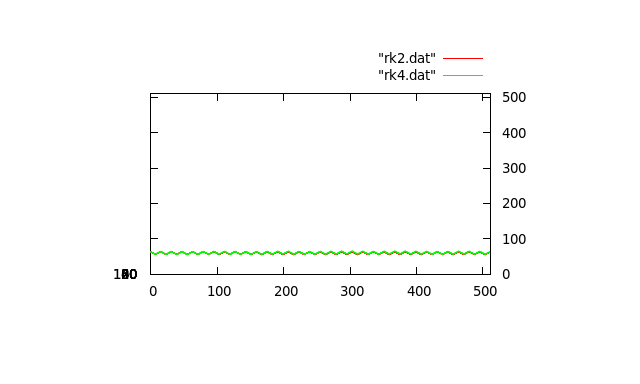
\includegraphics[width=80mm, height=50mm]{img/gnuplot-lines.png}
      \label{fig:2}
      \caption{Visualização no OpenGL do resultado dos algoritmos para um campo vetorial 512x512x128, com ponto inicial (0,64,64) e tamanho de passo 0.2, que representa a direção de retas mudando periodicamente.}
    \end{center}
  \end{figure}
\end{frame}

\begin{frame}
  \frametitle{Visualização}
  \framesubtitle{OpenGL}
  
    \begin{figure}
    \begin{center}
      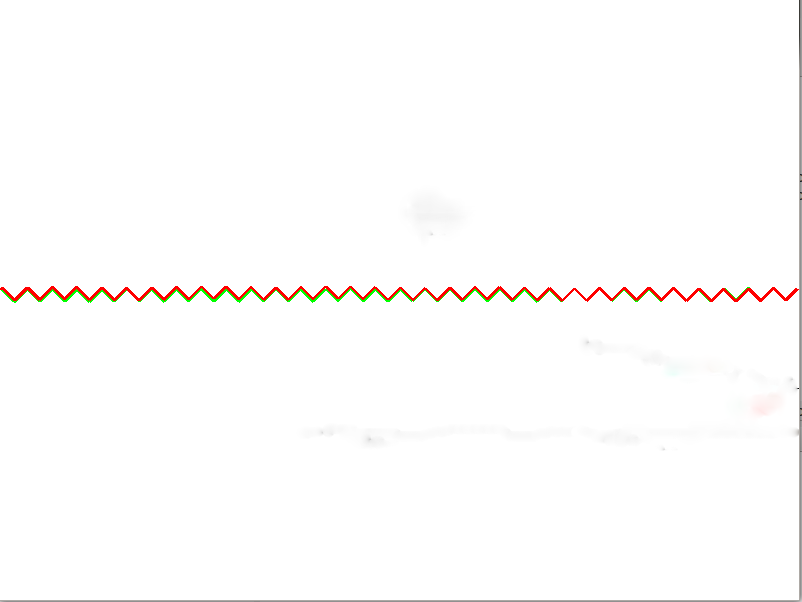
\includegraphics[width=80mm, height=50mm]{img/opengl-lines.png}
      \label{fig:2}
      \caption{Visualização no OpenGL do resultado dos algoritmos para um campo vetorial 512x512x128, com ponto inicial (0,64,64) e tamanho de passo 0.2, que representa a direção de retas mudando periodicamente. Podemos ver que a resolução é maior que com o gnuplot e que depois de muitas iterações o RK2 diverge mais rápido.}
    \end{center}
  \end{figure}
\end{frame}

\begin{frame}
  \frametitle{Visualização}
  \framesubtitle{VTK}
  \begin{figure}
    \begin{center}
      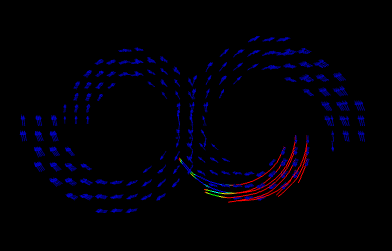
\includegraphics[width=78mm, height=50mm]{img/vtk.png}
      \label{fig:}
      \caption{Visualização através da implementação com a biblioteca VTK para um campo 32x32x32 representando a intersecção de duas hélices, com pontos iniciais na base de uma das hélices. Esta biblioteca permite facilmente visualizar o resultado (em vermelho) e os vetores do campo (em azul)}
    \end{center}
  \end{figure}
\end{frame}

\section{Conclusão}
\begin{frame}
  \frametitle{Conclusões}
  \framesubtitle{}

  \begin{itemize}
    \item A discretização de EDOs como campo campo vetorial e a adaptação do método de Runge-Kutta não comprometem, visualmente, a precisão do resultado;
    \item A implementação de um \textit{kernel} em CUDA e OpenCL que aplique o método foi comprovada como possível;
    \item Também foi comprovada como sendo muito mais rápida que uma implementação equivalente em C++ para CPU;
    \item Portanto, a tractografia em tempo real é possível através de CUDA e OpenCL.
  \end{itemize}
\end{frame}

\end{document}
